%\section{Human Resource Allocation}
%\label{DDHR}
%The first part of the project will involve a team of five specialists designing the five critical subsystems and one person designing the orbits of the swarm. The other four members will concentrate on the development of the software that will be used to assist the trade-off and verify the design. At later stages, some of the the software engineering personnel is heavily involved in designing proper algorithms for the processing of mission data, while others will be brought in to assist with detail design. 
%
%A schematic representation of the resource allocation can be found in figure \ref{fig:DDBBHR} on page \pageref{fig:DDBBHR}.
%
%\begin{figure}[ht!]
%\begin{center}
%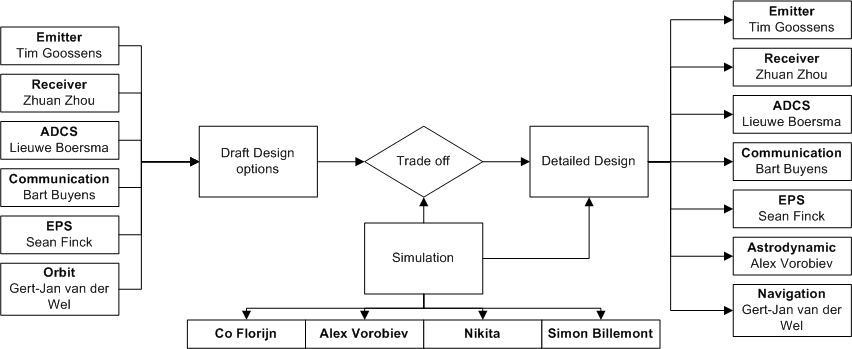
\includegraphics[width=0.9\textwidth]{chapters/img/DDBBHR.jpg}
%\label{fig:DDBBHR}
%\caption{Human resource allocation chart}
%\end{center}
%\end{figure}
%
%The table \ref{tab:RWD} on page \pageref{tab:RWD} gives the documentation distribution of each person on each chapter.

\begin{table}[ht!]
\centering
\scalebox{0.7}{
  
\begin{tabular}{|c|l|c|c|}
\hline
 Chapter & Documentation                      & Author & Checked by \\\hline 
 -       & Title Page                           & Alex   & \\\hline                  
 -       & Preface                              & Co, Team& \\\hline
 -       & List of Symbol                       &\\\hline
 -       & List of Acronyms                       &\\\hline
 -       & Abstract                             & Co, Bart &\\\hline
 1       & Introduction                         &\\\hline\hline
 2       & Project Management                   &\\\hline
 2.1     & \ -Resource Allocation               & Zhuan &\\\hline
 2.2     & \ -Budget Breakdown                  & Zhuan &\\\hline
 2.3     & \ -Operations and Logistic Concept Description&\\\hline
 2.4     & \ -Project Design and Development Logic & GJ &\\\hline
 2.5     & \ -Project Gantt Chart               & Lieuwe &\\\hline\hline
 3       & Mission Approach                     &\\\hline
 3.1     & \ -Function Flow Diagram             & Lieuwe, Zhuan & \\\hline
 3.2     & \ -Function Breakdown Structure      & Lieuwe, Zhuan &\\\hline
 3.3     & \ -H/W Block Diagram                 & Lieuwe, &\\\hline
 3.4     & \ -S/W Block Diagram                 &\\\hline
 3.5     & \ -Electrical Block Diagram          &\\\hline
 3.6     & \ -Data Handling Block Diagram       &\\\hline\hline
 4       & Risk Management                      &\\\hline\hline
 5       & Launch and Astrodynamic Characteristics & Alex &\\\hline
 5.1     & \ -Launch Segment                    & Alex &\\\hline
 5.2     & \ -Space Segment                     & Alex &\\\hline
 5.3     & \ -Space Environment and Shielding   & Alex &\\\hline\hline
 6       & Emitter                              &\\\hline
 6.1     & \ -OEP                               & Tim &\\\hline
 6.1.1   & \ \ -Principle of Diode Laser       & Tim &\\\hline
 6.1.2   & \ \ -Diode Pumped Laser Configuration & Tim &\\\hline
 6.1.3   & \ \ -Optical Characteristics        & Tim &\\\hline
 6.1.4   & \ \ -Diffraction                    & Tim &\\\hline  
 6.1.5   & \ \ -Thermal Control                & Tim, Lieuwe &\\\hline
 6.1.6   & \ \ -Laser Life Time Expectancy     & Tim &\\\hline
 6.1.7   & \ \ -Laser Focus Calculation        & Zhuan &\\\hline
 6.2     & \ -Navigation                        & GJ &\\\hline
 6.3     & \ -Communication                     & Bart &\\\hline
 6.4     & \ -ADCS                              & Lieuwe &\\\hline
 6.5     & \ -EPS                               & Sean &\\\hline
 6.6     & \ -Summary                           &\\\hline\hline
 7       & Receiver                             &\\\hline
 7.1     & \ -OEP                               & Zhuan &\\\hline
 7.1.2   & \ \ -SPAD Research                  & Tim, Zhuan &\\\hline
 7.1.3   & \ \ -Prism Design                   & Zhuan &\\\hline
 7.1.4   & \ \ -Summary                        & Zhuan &\\\hline
 7.1.5   & \ \ -Payload Cost Estimation        & Tim, Zhuan &\\\hline
 7.1.6   & \ -Navigation                        & GJ &\\\hline
 7.2     & \ -Communication                     & Bart &\\\hline
 7.3     & \ -ADCS                              & Lieuwe &\\\hline
 7.4     & \ -EPS                               & Sean &\\\hline
 7.5     & \ -Summary                           &\\\hline\hline
 8       & Data Validation                      & Programmer &\\\hline
 9       & Sustainable Development Strategy     &\\\hline
 10      & Compliance Matrix                    &\\\hline\hline
 -       & Others                               &\\\hline
 -       & \ -Catia Drawing                     & Lieuwe &\\\hline
 -       & \ -Latex Compile                     & Alex &\\
 \hline
\end{tabular}
}
\caption{Report writing distribution}
\label{tab:RWD}
\end{table}

%%%%%%%%%%%%%%%%%%%%%%%%%%%%%%%%%%%%%%%%%%%%%%%%%%%%%%%%%%%%%%%%%%%%%%%%%%%%%%%%%%%%%%%%%%%%%
%\section{Mass Budget Breakdown}
%\label{DDMBB}
%
%\begin{table}[ht!]
%\centering
%\begin{tabular}{|l|c|c|}
%\hline
%  & Author & Checked by \\\hline
%  & Author & Checked by \\\hline 
% \hline
%\end{tabular}
%\caption{Report writing distribution}
%\label{tab:RWD}
%\end{table}

%%%%%%%%%%%%%%%%%%%%%%%%%%%%%%%%%%%%%%%%%%%%%%%%%%%%%%%%%%%%%%%%%%%%%%%%%%%%%%%%%%%%%%%%%%%%%%
%\section{Cost Budget Breakdown}
%\label{blBudgetCost}
%The cost breakdown can be found in figure \ref{fig:costbreak} on page \pageref{fig:costbreak}. In this diagram, the cost is broken down into segments. This way it is easier to follow cost distribution down to all subsystems.
%
%Because of the nature of the system that is being designed - as a collection of satellites - it is very hard to make an accurate prediction of costs before critical decisions have been made. Most subsystem costs are mass driven, so design options create a large margin of error in early estimates. Furthermore, due to the high cost of actual production of individual satellites, a swarm is hard to predict without a rough idea of the number of space platforms. It is important to note that cost is also dependent on so called heritage factors. These factors allow for reduction of costs based on already existing designs. However, if some kind of new technology is used in a subsystem then this reduction cannot be used.
%
%Table \ref{tab:CostBreakdown} on page \pageref{tab:CostBreakdown} contains percentage estimations of all aspects covered in figure \ref{fig:costbreak}.
%
%
%\begin{table*}[htbp]
%	\centering
%
%% Table generated by Excel2LaTeX from sheet 'Sheet1'
%\begin{tabular}{p{10cm} | c | c }
%
%   \textbf{SEGMENT} & \textbf{$\%$ OF PARENT} & \textbf{$\%$ OF TOTAL} \\ \hline \hline
%
%\textsl{Space Segment} &          &       30   \\ \hline
%
%      \hspace{1.0cm}RDTE &         30 &   9       \\ \hline
%
%   \hspace{2.0cm}Payload &         26 &     2.3     \\
%
%       \hspace{2.0cm}Bus &         52 &     4.7    \\ \hline
%
% \hspace{2.5cm}Structure &         24&      1.1    \\
%
%  \hspace{2.5cm}Thermal &         2 &       0.1   \\
%
%      \hspace{2.5cm}EPS &         22 &      1    \\
%
%\hspace{2.5cm}Communications &         38 &      1.8    \\
%
%      \hspace{2.5cm}ADCS &         14 &     0.7     \\ \hline
%
%       \hspace{2.0cm}IAT &         0 &         0 \\
%
% \hspace{2.0cm}Program Level &         22 &       2   \\ \hline
% \hspace{2.5cm}Program Management &         20 &      0.4    \\
% \hspace{2.5cm}Systems Engineering &         40 &     0.8     \\
% \hspace{2.5cm}Product Assurance &         20 &       0.4   \\
% \hspace{2.5cm}System Evaluation &         20 &       0.4   \\ \hline
%
%        \hspace{2.0cm}GSE &         4 &      0.4    \\
%
%      \hspace{2.0cm}LOOS &         0 &         0 \\ \hline
%
%  \hspace{1.0cm}Software &         25 &         7.5 \\
%
%\hspace{1.0cm}Production &         45 &         13.5 \\ \hline
%
%       \hspace{2.0cm}TFU &         10-30 &       1.4-4.8   \\ \hline
%
%   \hspace{2.5cm}Payload &         20 &       0.3-0.8   \\
%
%       \hspace{2.5cm}Bus &         45 &        0.6-1.8  \\ \hline
%
% \hspace{3.0cm}Structures &         24 &       0.1-0.4   \\
%
%   \hspace{3.0cm}Thermal &         5 &         0.04-0.12 \\
%
%       \hspace{3.0cm}EPS &         20 &        0.1-0.4  \\
%
%\hspace{3.0cm}Communications &         18 &      0.1-0.3    \\
%
%      \hspace{3.0cm}ADCS &         28 &         0.2-0.5 \\ \hline
%
%       \hspace{2.5cm}IAT &         14&         0.2-0.6 \\
%
%\hspace{2.5cm}Program Level &         13 &         0.2-0.5 \\ \hline
% \hspace{3.0cm}Program Management &         30 &       0.05-0.16   \\
% \hspace{3.0cm}Systems Engineering &         20 &        0.04-0.11  \\
% \hspace{3.0cm}Product Assurance &         30 &       0.05-0.16   \\
% \hspace{3.0cm}System Evaluation &         20 &       0.04-0.11   \\ \hline
%
%       \hspace{2.5cm}GSE &         0 &          0\\
%
%      \hspace{2.5cm}LOOS &         5 &         0.07-0.2 \\ \hline
%
%     \hspace{2.0cm}Swarm &         70-90 &         9.5-12 \\ \hline
%
%\textit{Launch Segment} &         &         5-10 \\ \hline
%
%  \hspace{1.0cm}Launcher &         100 &        5-10  \\ \hline
%
%\textit{Ground Segment} &          &     20     \\ \hline
%
%\hspace{1.0cm}First Ground Station &         25 &      5    \\
%
%\hspace{1.0cm}Consecutive Ground Stations &         55 &     11     \\
%
%\hspace{1.0cm}Software &         20 &     4     \\ \hline
%
%\textit{Operations and Maintenance} &          &        45  \\ \hline
%
%\hspace{1.0cm}Operations and support of ground stations &         100 &   45       \\
%	
%\end{tabular} 
%\caption{Cost budget breakdown estimations}
%	\label{tab:CostBreakdown} 
%\end{table*}
%
%\begin{figure}[ht!]
%\begin{center}
%
%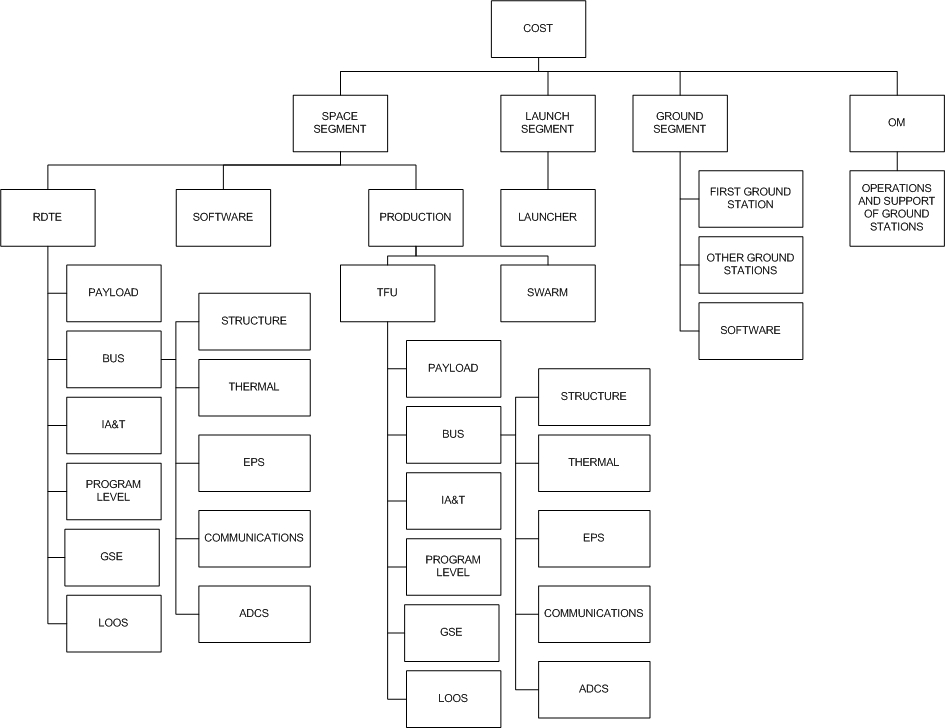
\includegraphics[height=0.8\textwidth,angle=90]{chapters/img/costbreakdown.jpg}
%\caption{Cost Budget Breakdown Structure}
%\label{fig:costbreak}
%\end{center}
%\end{figure}


